\chapter{Architectural Design}

\section{Overview}
We chose to design the Students\&Companies (S\&C) web application using a three-tier architecture with remote presentation. These three tier correspond to a client tier, application tier and data tier. The client (presentation) tier serves the needs of both students, companies and universities using the S\&C platform. The application layer is the one that processes user request, performs statistical analysis and interacts with the internal data tier. The data tier is responsible for data management and storage. It handles all database operations, including data retrieval, updates, and management. To better improve and ensure load distribution and scalability, it was chosen to implement a load balancer between the client and application layer, in particular inside the web server.

A 3-tier architecture is suitable for a career service application as it makes the system easier to manage and scale. It ensures reliability through load balancing, which helps handle high traffic during peak usage. This architecture supports advanced features like job matching and analytics, integrates well with cloud services, and provides flexibility for future updates, such as adding mobile apps or AI tools. Its structure also improves security by isolating sensitive data in the database layer.

The S\&C architecture specializes in three different groups of components each with its own characteristics and responsibilities:
\begin{enumerate}
    \item \textbf{Presentation layer:} The Presentation (client) Tier is the application's front end, managing the user interface and interactions for data input and display. Its goal is to display data, collect inputs and provide a seamless user experience. 
    \item \textbf{Application layer:} It handles tasks like user authentication, recommendation matching algorithms, managing user accounts, handling notifications, and communication between the user interface and the database.
    \item \textbf{Data layer}: Stores and manages critical data such as user profiles, student's CVs, project descriptions, and application history. It ensures data security and efficient retrieval for real-time use in the application.
\end{enumerate}

\begin{figure}[H]
    \centering
    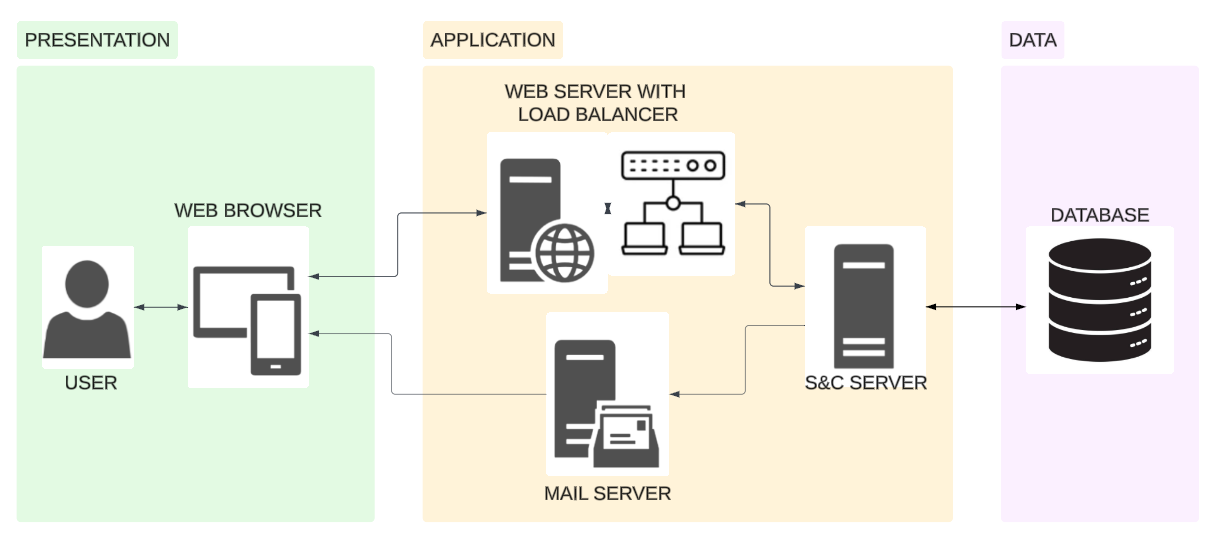
\includegraphics[width=0.8\linewidth]{DD//Images/3tier.png}
    \caption{High level architecture }
\end{figure}

\section{Component view} 

\subsection{Component diagram}

\begin{figure}[H]
    \centering
    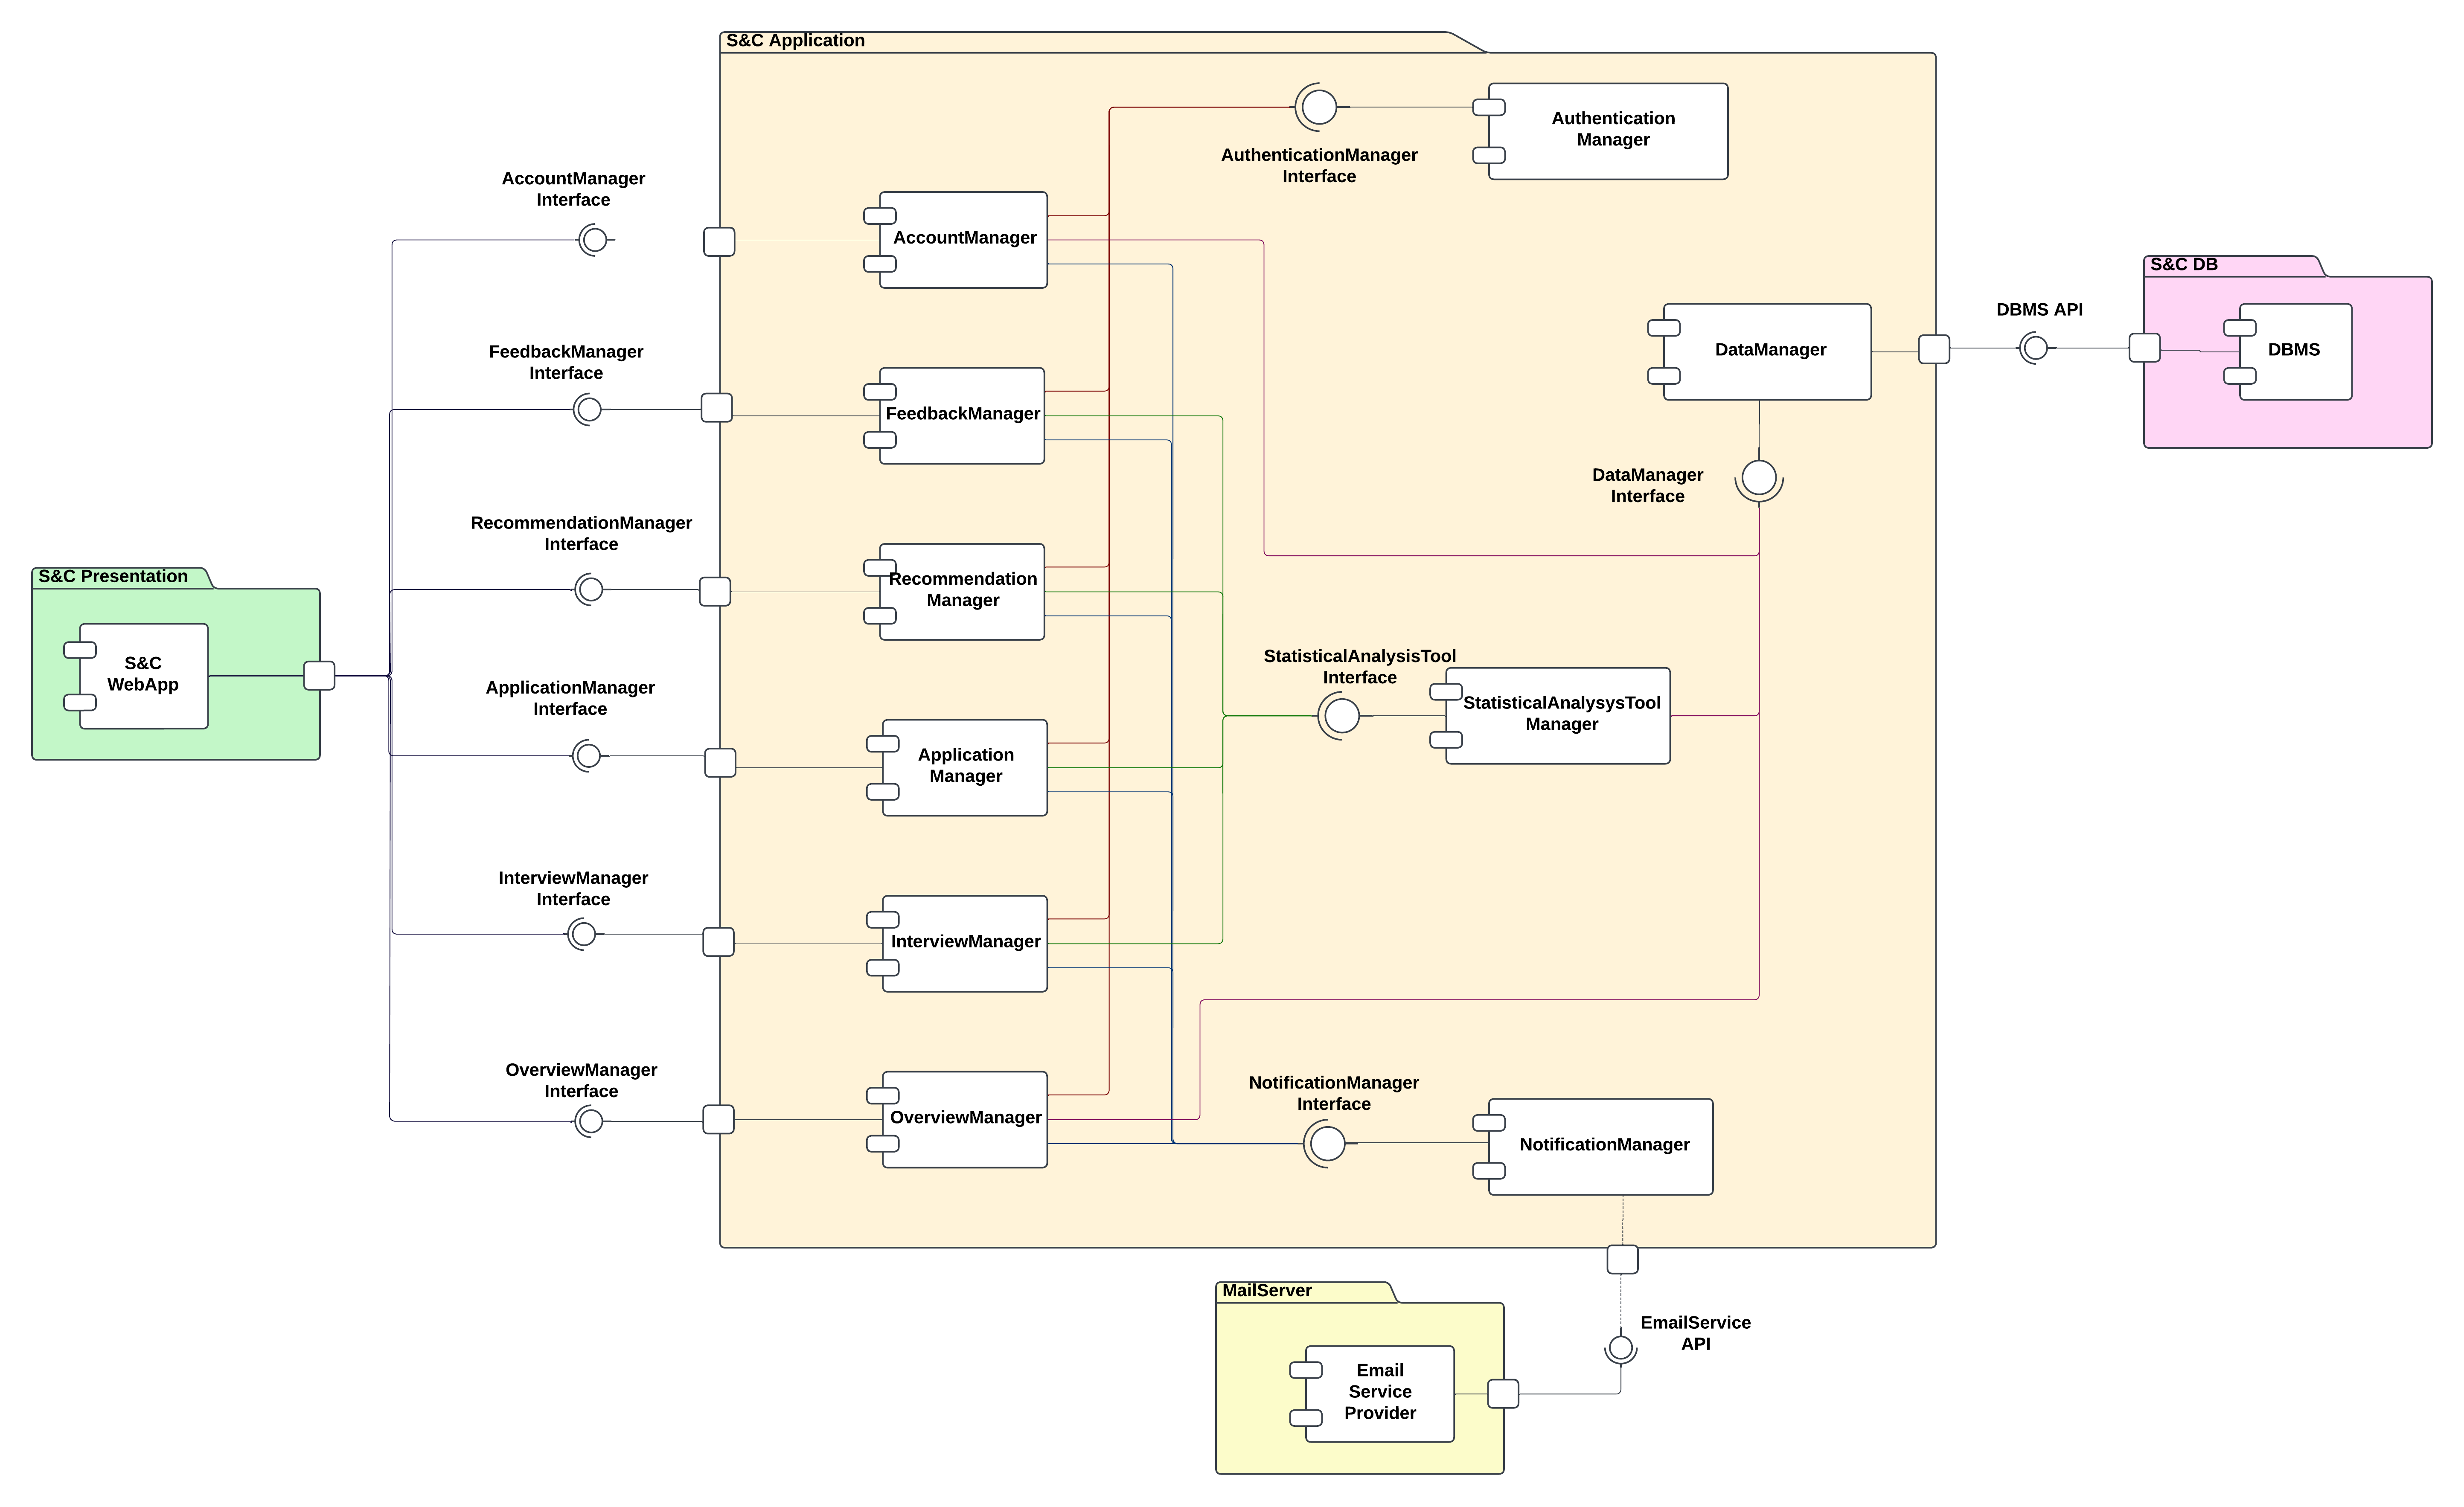
\includegraphics[width=1\linewidth]{DD//Images/ComponentDiagram.png}
    \caption{Component Diagram }
\end{figure}

Figure 2.2 presents a detailed diagram illustrating the components that constitute our application. Below is an explanation of each component and its purpose.

\begin{itemize}
    \item \textbf{WebApp:} The WebApp serves as the primary interface for all users: students, companies, and universities, allowing them to interact with the application via their web browser. User requests are processed and sent to the appropriate backend components through the defined interfaces.
    \item \textbf{Account Manager:} The Account Manager is a backend module responsible for managing all aspects of account registration, login, and user data. It handles the creation of different user profiles and ensures the validity of the submitted data. The Account Manager communicates with the Statistical Analysis Tool Manager to notify it of any updates to user data and works with the Notification Manager to send notifications to users as needed. To save the new user's data, the Account Manager interacts with the Data Manager to store the information in the database. However, before performing any database operations, the Account Manager first requests permission from the Authentication Manager to ensure that the user is authenticated and authorized to perform the action.
    \item \textbf{Feedback Manager:}The Feedback Manager is responsible for gathering user feedback from both students and companies. It proactively requests feedback when needed through the Notification Manager, ensuring timely user engagement. This module collaborates with the Statistical Analysis Tool by providing updated feedback data, enabling continuous improvement of the recommendation system and analysis capabilities.
    \item \textbf{Recommendation Manager:} The Recommendation Manager is the module that is responsible for requesting and receiving internship matches between students and projects from the Statistical Analysis Tool. After obtaining the matches, it communicates the results to the Notification Manager, which then notifies the involved users about the recommended opportunities.
    \item \textbf{Application Manager:} The Application Manager handles student applications in three scenarios: when a student proactively applies for an internship they are interested in, when a student either accepts a recommendation, and when responds to an invitation from a company that has previously accepted the system's recommendation. After processing the applications, it communicates with the Notification Manager to notify both students and companies about the submitted applications. Additionally, it interacts with the Statistical Analysis Tool to provide data for further analysis and improvement of the recommendation system.
    \item \textbf{Interview Manager:} The Interview Manager oversees the entire interview and final selection process. It communicates with the Notification Manager to keep both students and companies informed about new developments throughout the process. Additionally, it interacts with the Statistical Analysis Tool to provide data, such as information on who was selected for the job, helping to refine the system and adjust parameters for future job recommendations.
    \item \textbf{Overview Manager:} The Overview Manager is responsible for monitoring ongoing internships. It communicates with the Notification Manager to keep universities, students, and companies involved in the project updated on progress. Additionally, it interacts with the Authentication Manager to obtain permission for accessing data, and then works with the Data Manager to insert and register the relevant updates.
    \item \textbf{StatisticalAnalysisTool Manager:} The Statistical Analysis Tool Manager is responsible for generating matches between students and internship projects based on student CVs and project descriptions. It also provides suggestions to students for improving their CVs and to companies for enhancing their project descriptions. These tasks are performed using a recommendation system powered by AI and machine learning. The tool is continuously refined through feedback from both students and companies about its previous recommendations. It communicates with the Data Manager to access the necessary data, with prior authentication provided by the Authentication Server.
    \item \textbf{Notification Manager:} The Notification Manager is responsible for sending notifications to all users across various channels. It interacts with the email service API to send email notifications and also delivers real-time updates directly within the web app. When delivering notifications through the app, it follows the chain of requests, processing them in reverse order to ensure that all relevant parties receive the appropriate updates.
    \item \textbf{Authentication Manager:} The Authentication Manager is responsible for managing access rights to data, ensuring that users can perform read or write operations based on their role and permissions.
    \item \textbf{Data Manager:} The Data Manager is responsible for managing and storing all data within the system. It handles data retrieval, updates, and ensures that information is accurately recorded and stored. The module interacts with other components to provide the necessary data for operations while maintaining data integrity and security.
    \item \textbf{Email Service Provider:} The Email Service Provider is an external module that interacts with the Notification Manager to send email notifications to users. It handles the delivery of emails for various events, such as application updates, interview schedules, and system alerts.
    \item \textbf{DBMS:} The DBMS (Database Management System) is responsible for managing and organizing the system's database. It handles data storage, retrieval, and manipulation, ensuring data integrity, security, and efficient access. The DBMS interacts with other modules to support operations such as user authentication, data analysis, and application management, storing and managing all relevant information within the system.
    
\end{itemize}

\section{Deployment view}

\section{Runtime view}

All the sequence diagrams described in the Requirements Analysis and Specification Document (RASD) will be elaborated in greater detail. In this expanded version, we will identify and specify the individual components of the application that are utilized to fulfill each specific functionality. 

Here below we will include an explanation of how each application component contributes to the implementation of the corresponding functionality. By doing so, we hope to provide a clearer understanding of the interaction between various components and their roles in achieving the described features and requirements.

Spiegazione su di cosa si occupa ogni component e poi tutti i sequence diagram..

\textbf{UC1: Student creates an account}
WebApp, AccountManager, Authentication manager, DataManager, DBMS, NotificationManager, EmailServiceProvider

\textbf{UC2: Company creates an account}
WebApp, AccountManager, Authentication manager, DataManager, DBMS, NotificationManager, EmailServiceProvider

\textbf{UC3: Student searches and applies for an internship}
WebApp, AccountManager, Authentication manager, ApplicationManager, StatisticalAnalysisToolManager, DataManager, DBMS, NotificationManager, EmailServiceProvider

\textbf{UC4: Student recieves an internship recommendation}
WebApp, AccountManager, Authentication manager, RecommendationManager, ApplicationManager, StatisticalAnalysisToolManager, DataManager, DBMS, NotificationManager, EmailServiceProvider

\textbf{UC5: Company recieves a student's recommendation}
WebApp, AccountManager, Authentication manager, RecommendationManager, ApplicationManager, StatisticalAnalysisToolManager, DataManager, DBMS, NotificationManager, EmailServiceProvider

\textbf{UC6: Interview}
WebApp, AccountManager, Authentication manager, ApplicationManager, StatisticalAnalysisToolManager, InterviewManager, DataManager, DBMS, NotificationManager, EmailServiceProvider

\textbf{UC7: User leaves feedback}
WebApp, AccountManager, Authentication manager, FeedbacknManager, StatisticalAnalysisToolManager, DataManager, DBMS, NotificationManager, EmailServiceProvider

\textbf{UC8: Student recieves suggestion on CV}
WebApp, AccountManager, Authentication manager, StatisticalAnalysisToolManager, DataManager, DBMS, NotificationManager, EmailServiceProvider

\textbf{UC9: Company recieves suggestion on project description}
WebApp, AccountManager, Authentication manager, StatisticalAnalysisToolManager, DataManager, DBMS, NotificationManager, EmailServiceProvider

\textbf{UC10: User makes a complaint}
WebApp, AccountManager, Authentication manager, OverviewManager, StatisticalAnalysisToolManager, DataManager, DBMS, NotificationManager, EmailServiceProvider






\section{Component interfaces}
The Component Interfaces here described are the ones exposed in the components. Only the most relevant method parameters and methods
are shown.

\begin{itemize}
\item \textbf{Account Manager Interface}
    \begin{itemize}
    \item \textbf{registerUserAsStudent(string Email, string Name, data BirthDate, string LocationBirth, string Password) : boolean AccountCreated}

    This method takes all the data in input and contacts the DataManager to register a new StudentUser in the system.

    \item \textbf{registerUserAsCompany(string Email, string CompanyName, string LocationAddress, string Password) : boolean AccountCreated}
    
    This method takes all the data in input and contacts the DataManager to register a new CompanyUser in the system.

    \item \textbf{registerUserAsUniversity(string Email, string UniversityName, string LocationAddress, string Password) : boolean AccountCreated}
    This method takes all the data in input and contacts the DataManager to register a new UniversityUser in the system.

    \item \textbf{loginUser(string Email, string Password) : boolean LoginSuccessful}
    
    This method takes the user's email and password, check whetere they are registered and if they are it logs them into their account

    \item \textbf{insertCv(CV Cv): boolean Inserted}
    
    This method allows a StudentUser to upload their Cv on their profile. 

    \item \textbf{deleteCv(): boolean Deleated}
    
    This method allows a StudentUser to delete their Cv from their profile.
    
    \item \textbf{insertProjectDescription(string ProjectDescription): booleand Inserted}
    This method allows a CompanyUser to upload a new project description on their profile.

    \item \textbf{deleteProjectDescription(string ProjectName): booleand Deleted}
    
    This method allows a CompanyUser to delete a project description from their profile.

    \item \textbf{modifyAttribute(string AttributeName, string NewValue): boolean Modified}
    
    This method allows users to modify any data present on their profile.
    \end{itemize}

\item \textbf{Authentication Manager Interface:}
\begin{itemize}
\item \textbf{authenticateUser(string Email, string Password) : boolean IsAuthenticated}  
This method verifies the provided email and password against the stored credentials. If the credentials are valid, it returns `true`; otherwise, it returns `false`.

\item \textbf{authorizeAction(string Email, string Action) : boolean IsAuthorized}  
This method determines whether the specified user has the necessary permissions to perform the given action. It returns `true` if the action is allowed, otherwise `false`.


\end{itemize}

\item \textbf{Feedback Manager Interface}
    \begin{itemize}
    \item \textbf{requestFeedback(string UserType, string FeedbackType): boolean Requested}

    This method sends a request for feedback to the specified user type (e.g., student or company) using the Notification Manager. The FeedbackType determines the nature of the feedback requested.

    \item \textbf{submitFeedback(string UserId, string FeedbackContent): boolean Submitted}

    This method allows users to submit their feedback. The content is processed and forwarded to the Statistical Analysis Tool for further use.

    \item \textbf{getFeedbackHistory(string UserId): list FeedbackList}

    This method retrieves the history of feedback provided by a specific user for review or analysis purposes.

    \item \textbf{updateStatisticalAnalysisTool(string FeedbackData): boolean Updated}

    This method sends the collected feedback to the Statistical Analysis Tool, enabling continuous refinement of the recommendation system.

    \item \textbf{notifyFeedbackUpdate(string UserId, string FeedbackStatus): boolean Notified}

    This method communicates with the Notification Manager to inform users about the status or impact of their feedback submissions.
    \end{itemize}
    
\item \textbf{Application Manager Interface:}
\begin{itemize}
    \item \textbf{submitApplication(string UserId, string InternshipId): boolean Submitted}

    This method allows a student to submit an application for a specified internship. It processes the application and records it in the system.

    \item \textbf{acceptRecommendationStudent(string UserId, string RecommendationId): boolean Accepted}

    This method processes a student's acceptance of a recommendation provided by the system and creates an application for the corresponding internship.

     \item \textbf{acceptRecommendationCompany(string UserId, string RecommendationId): boolean Accepted}

    This method processes a company's acceptance of a recommendation provided by the system and creates an invitation for the Student for the corresponding internship.

    \item \textbf{respondToInvitation(string UserId, string InvitationId): boolean Responded}

    This method allows a student to respond to an invitation from a company and generates an application if the invitation is accepted.

    \item \textbf{notifyApplicationUpdate(string UserId, string CompanyId, string ApplicationStatus): boolean Notified}

    This method communicates with the Notification Manager to inform both the student and the company about updates or changes to the application status.

    \item \textbf{sendDataToStatisticalAnalysisTool(string ApplicationData): boolean Sent}

    This method sends processed application data to the Statistical Analysis Tool to assist in refining the recommendation system and improving future matches.
    \end{itemize}

\item \textbf{Interview Manager Interface:}
\begin{itemize}
    \item \textbf{createAssessmentForum(string CompanyId, string UserId, string AssessmentDetails): boolean Created}

    This method allows a company to create a forum for conducting a prior assessment with a student. The forum includes assessment details and discussion tools for evaluations.

    \item \textbf{resolveAssessment(string ForumId, string ResolutionDetails): boolean Resolved}

    This method finalizes the outcome of a prior assessment conducted in the forum and records the resolution in the system.

    \item \textbf{evaluateAssessment(string ForumId, string EvaluationFeedback): boolean Evaluated}

    This method records feedback and evaluations on the assessment process, providing insights for both the student and the company.
    
    \item \textbf{scheduleInterview(string UserId, string CompanyId, datetime InterviewDate): boolean Scheduled}

    This method schedules an interview between a student and a company and records the details in the system.

    \item \textbf{updateInterviewStatus(string InterviewId, string Status): boolean Updated}

    This method allows updating the status of an interview (e.g., scheduled, completed, canceled) and ensures the system reflects the current progress.

    \item \textbf{finalizeSelection(string CompanyId, string UserId): boolean Finalized}

    This method records the final selection decision made by the company and updates the relevant data.

    \item \textbf{notifyInterviewUpdate(string UserId, string CompanyId, string NotificationMessage): boolean Notified}

    This method communicates with the Notification Manager to keep both the student and the company updated about any changes or developments in the interview process.

    \item \textbf{sendSelectionDataToStatisticalAnalysisTool(string SelectionData): boolean Sent}

    This method forwards data on the final selection process to the Statistical Analysis Tool to refine future recommendations and adjust job parameters.
    \end{itemize}



\item \textbf{Overview Manager Interface:}
\begin{itemize}
    \item \textbf{trackInternshipProgress(string InternshipId): map ProgressData}

    This method retrieves the current progress data for a specific internship, including details about the student, company, and related activities.

    \item \textbf{updateInternshipStatus(string InternshipId, string StatusUpdate): boolean Updated}

    This method updates the status of an ongoing internship (e.g., in progress, paused, completed) and records the changes in the system.

    \item \textbf{logInternshipUpdate(string InternshipId, string UpdateDetails): boolean Logged}

    This method registers detailed updates regarding the internship in the database. It communicates with the Authentication Manager for permission and the Data Manager to store the data.

    \item \textbf{uploadComplaint(string InternshipId, string UserId, string ComplaintDetails): boolean Uploaded}

    This method allows students or companies to file a complaint about the internship. The complaint is logged in the system for review and resolution by the university.

    \item \textbf{resolveComplaint(string InternshipId, string ComplaintId, string ResolutionDetails): boolean Resolved}

    This method allows universities to resolve complaints raised during the internship. Resolutions are documented and communicated back through the app.

    \item \textbf{reportComplaintOutcome(string InternshipId, string ComplaintId): boolean Reported}

    This method updates the system with the outcome of externally resolved complaints, ensuring all data remains centralized and accessible.

    \item \textbf{manageFeedback(string InternshipId, string FeedbackContent): boolean Managed}

    This method processes feedback submitted by students or companies about the internship and stores it in the system for future reference.

    \item \textbf{contactParticipant(string InternshipId, string ParticipantId, string MessageContent): boolean Contacted}

    This method enables the university to directly contact a student or company involved in the internship by sending a message through the app.

    \item \textbf{notifyProgressUpdate(string UserId, string NotificationMessage): boolean Notified}

    This method interacts with the Notification Manager to inform universities, students, and companies about any new updates or changes in the internship.

    \item \textbf{sendProgressDataToStatisticalAnalysisTool(string ProgressData): boolean Sent}

    This method provides ongoing internship data to the Statistical Analysis Tool, enabling analysis and improvement of internship processes.
    \end{itemize}
    

\item \textbf{StatisticalAnalysisTool Manager Interface:}
\begin{itemize}
    \item \textbf{generateMatches(string StudentId, string ProjectId): list Matches}

    This method generates a list of potential matches between students and internship projects based on student CVs and project descriptions using the recommendation system.

    \item \textbf{suggestCvImprovements(string StudentId, CV Cv): list Suggestions}

    This method analyzes a student's CV and provides personalized suggestions for improvements to enhance their profile and compatibility with internship opportunities.

    \item \textbf{suggestProjectImprovements(string CompanyId, string ProjectDescription): list Suggestions}

    This method evaluates a company's project description and provides recommendations for making it more appealing and clear to potential candidates.

    \item \textbf{refineRecommendations(string FeedbackData): boolean Refined}

    This method processes feedback received from students and companies about previous recommendations to update and improve the recommendation algorithm.

    \item \textbf{analyzeSelectionData(string SelectionData): boolean Analyzed}

    This method evaluates data on selected candidates to refine parameters and optimize future recommendations.

    \item \textbf{fetchData(string DataRequest): map Data}

    This method interacts with the Data Manager to retrieve necessary data for analysis, ensuring access permissions are obtained through the Authentication Server.

    \item \textbf{updateRecommendationParameters(string Parameters): boolean Updated}

    This method adjusts the recommendation system's parameters based on new data or trends observed during analysis.

    \item \textbf{notifyFeedbackProcessed(string UserId, string NotificationMessage): boolean Notified}

    This method interacts with the Notification Manager to inform users that their feedback has been processed and incorporated into system improvements.
    \end{itemize}


\item \textbf{Notification Manager Interface:}
\begin{itemize}
    \item \textbf{sendAccountNotification(userEmail: String, notificationType: String, message: String): String message}

    This method is used to send notifications related to account activities, such as registration confirmations, password updates, or account deactivations. It’s typically called by the Account Manager.
    The method takes the userEmail (the ID of the user to notify), a notificationType (like "Registration"), and a message containing the notification content. The message is both sent by email through the notification manager and The Account Manager receives the formatted message through the backward chain and passes it along to the WebApp, where it’s displayed to the user in the notification page.
    \item \textbf{sendFeedbackNotification(userEmail: String, feedbackType: String, message: String): String message
}

    This method is used to send notifications requesting or acknowledging user feedback, such as a prompt to review an internship or provide suggestions for improvement. It’s typically called by the Feedback Manager.
    The method takes the userEmail (the email of the user to notify), a feedbackType (like "InternshipFeedback"), and a message containing the notification content. The message is sent by email through the Notification Manager, and the Feedback Manager receives the formatted message through the backward chain and passes it along to the WebApp, where it is displayed to the user to encourage engagement.
    \item \textbf{sendRecommendationNotification(userEmail: String, recommendationDetails: String): String message
}

    This method is used to send notifications about internship recommendations to students or companies, informing them about relevant matches. It’s typically called by the Recommendation Manager.
    The method takes the userEmail (the email of the user to notify) and recommendationDetails (like "You have been recommended for the Software Engineer position at TechCorp"). The message is sent by email through the Notification Manager, and the Recommendation Manager receives the formatted message through the backward chain and passes it along to the WebApp, where the user is notified about the recommendation on their dashboard.
    \item \textbf{sendApplicationNotification(userEmail: String, applicationStatus: String, message: String): String message}

    This method is used to notify users about updates related to their internship applications, such as submission confirmations, acceptance, or rejections. It’s typically called by the Application Manager.
    The method takes the userEmail (the email of the user to notify), an applicationStatus (like "Submitted" or "Accepted"), and a message detailing the update. The message is sent by email through the Notification Manager, and the Application Manager receives the formatted message through the backward chain and passes it along to the WebApp, where the user sees the application update on the notification page.
    \item \textbf{sendInterviewNotification(userEmail: String, interviewDetails: String): String message}

    This method is used to notify users about interview-related updates, such as scheduling, rescheduling, or cancellations. It’s typically called by the Interview Manager.
    The method takes the userEmail (the email of the user to notify) and interviewDetails (like "Your interview is scheduled for July 5th at 3:00 PM"). The message is sent by email through the Notification Manager, and the Interview Manager receives the formatted message through the backward chain and passes it along to the WebApp, where the user sees the interview details on their notification page.
    \item \textbf{sendOverviewNotification(userEmail: String, progressUpdate: String): String message}

    This method is used to notify users about updates on the progress of ongoing internships, ensuring students, universities, and companies are informed about important milestones. It’s typically called by the Overview Manager.
    The method takes the userEmail (the email of the user to notify) and a progressUpdate (like "Your student has reached 80\% of the internship goals"). The message is sent by email through the Notification Manager, and the Overview Manager receives the formatted message through the backward chain and passes it along to the WebApp, where it’s displayed on the notification page for relevant users.

    \item \textbf{sendGeneralNotification(userEmail: string, toUserIds: List[String], message: String): String message}
    
    This method is used for sending generic notifications that don’t fit into other specific categories. It supports notifications across various channels and can target multiple users simultaneously. It’s called by any module requiring an ad hoc notification.
    The method takes a list of toUserEmails (the emails of the users to notify), a channel (like "email" or "app"), and a message containing the content to be sent. The message is sent through the specified channel by the Notification Manager, and the calling module receives the formatted message through the backward chain and passes it along to the WebApp, where it’s displayed in the user’s notification area.


\end{itemize}


\item \textbf{Data Manager:}
\begin{itemize}
    
\item \textbf{saveRecord(string TableName, map<string, string> Data) : boolean RecordSaved}  

This method saves a new record in the specified table. It returns `true` if the record is successfully stored.

\item \textbf{fetchRecord(string TableName, string Condition) : map<string, string> FetchedRecord}  

This method retrieves a single record from the specified table that matches the provided condition. Returns the record as a key-value map.

\item \textbf{fetchAllRecords(string TableName, string Condition) : list<map<string, string>> RecordsList} 

This method retrieves all records from the specified table that match the provided condition. Returns the data as a list of key-value maps.

\item \textbf{updateRecord(string TableName, map<string, string> Updates, string Condition) : boolean RecordUpdated}  

This method updates records in the specified table based on the condition provided. Returns `true` if the update is successful.

\item \textbf{deleteRecord(string TableName, string Condition) : boolean RecordDeleted}  

This method deletes records from the specified table that match the provided condition. Returns `true` if the deletion is successful.


\item \textbf{provideDataAccess(string ModuleName, string DataRequest) : map<string, string> AccessedData}  
This method grants secure data access to a specific module, returning the requested data while enforcing access control policies.

\end{itemize}

\item \textbf{Email Service Provider: }
\begin{itemize}
\item \textbf{sendEmail(string SenderEmail, string RecipientEmail, string Subject, string Body) : boolean EmailSent, string EmailId} 

This method sends an email to the specified recipient with the provided subject and body content. Returns `true` if the email is successfully sent.

\item \textbf{sendTemplatedEmail(string SenderEmail, string RecipientEmail, string TemplateName, map<string, string> TemplateData) : boolean EmailSent, string EmailId}  

This method sends an email using a predefined template. It takes the template name and a mapping of dynamic data to populate the template fields.

\item \textbf{trackEmailDelivery(string EmailId) : string DeliveryStatus} 

This method checks the delivery status of a previously sent email using its unique email ID. It returns statuses such as "Delivered," "Failed," or "Pending."

\item \textbf{configureEmailSettings(string SMTPServer, int Port, string SenderEmail, string SenderPassword) : boolean SettingsConfigured}  

This method configures the SMTP settings for sending emails, including the server address, port, sender email, and authentication details.

\item \textbf{validateEmailAddress(string EmailAddress) : boolean IsValid}  

This method checks whether the given email address is in a valid format and can be used for sending emails.

\item \textbf{resendFailedEmails(string[] FailedEmailIds) : boolean Resent}  
This method retries sending emails that previously failed to be delivered. Returns `true` if all retries are successful.
\end{itemize}

\item \textbf{DBMS:}
\begin{itemize}
\item \textbf{postData(string TableName, map<string, string> Data) : boolean IsStored} 

This method inserts the provided data into the specified table within the database. Returns `true` if the operation is successful.

\item \textbf{getData(string Query) : list<map<string, string>> RetrievedData}  

This method executes the provided query to fetch data from the database. It returns the results as a list of records.

\item \textbf{updateData(string TableName, map<string, string> Updates, string Condition) : boolean IsUpdated}

This method updates records in the specified table based on the condition provided. Returns `true` if the update is successful.

\item \textbf{deleteData(string TableName, string Condition) : boolean IsDeleted}  

This method removes records from the specified table that match the provided condition. Returns `true` if the deletion is successful.

\item \textbf{manageAccessControl(string UserId, string[] Permissions) : boolean AccessManaged}  

This method updates access control policies for a specific user by assigning or revoking permissions.

\end{itemize}
\end{itemize}


\section{Selected architectural styles and patterns}
\section{Other design decisions }
